% --------------------------------------------------------------------- %
% Model adapted by volunteer student João Antonio Teixeira Sucupira     %
% Supervision by Prof. Daniel Fernando Pigatto                          %
% Graduate Program in Applied Computing (PPGCA)                         %
% Federal University of Technology - Paraná (UTFPR)                     %
% --------------------------------------------------------------------- %

\documentclass{if-beamer}

\usepackage{array}
\usepackage{graphicx}
\usepackage{hyperref}
\usepackage{subfigure}
\usepackage{amsmath}





% --------------------------------------------------- %
%                  Presentation info                  %
% --------------------------------------------------- %
\title[NMF Overview Slides]{\textbf{SUAS Detection and Classification}}
\subtitle{Classical and Deep Learning Based Approaches to Signal Analysis}
\author[MMD, AC, GE]{\small \textbf{[CONTROLLED UNCLASSIFIED]}}
\institute[AFRL]{
    
\includegraphics[width=2cm]{images/afrl_logo.png}\\
    \small \textit{US Air Force Research Laboratory} \\
    \small \textit{Information Directorate}
}
\date{\today}
\logo{
\includegraphics[scale=.2, clip]{}
}
\subject{Presentation subject} % metadata
%trim={<left> <lower> <right> <upper>}
\graphicspath{{figuras/}}
% --------------------------------------------------- %
%                    Title + Schedule                 %
% --------------------------------------------------- %

\begin{document}

\begin{frame}
  \titlepage
\end{frame}

\begin{frame}{Agenda}
  \tableofcontents
\end{frame}

% --------------------------------------------------- %
%                      Presentation                   %
% --------------------------------------------------- %

%%%%%%%%%%%%%%%%%%%%%%%%%%%%%%%%%%%%%%%%%%%%%%%%%%%%%%%%%%%%%

\section{Introduction}


\begin{frame}{Motivation}

    \begin{itemize}
        \item Detection and classification of commercially available SUAS devices presents great difficulties 
        \item Audio signals recorded in real-world scenarios contain noise from various sources which increases the difficulty of identifying the presence of a UAS
        \item An automated, robust audio separation algorithm increases the likelihood of successful classification via supervised machine learning approaches
    \end{itemize}

\end{frame}

\begin{frame}{Digitization + Documentation}

    \begin{itemize}
        \item Streamlined workflow, centralized code, and compiled data via \href{https://github.com/ale-chen/afrl-uav-detection}{\textcolor{blue}{GitHub}} and Google Drive
        \item \href{https://github.com/ale-chen/afrl-uav-detection/blob/52835d45078ce6fe929cc821cafe20e7df242115/noise_subtraction/audioSeparation.ipynb}{\textcolor{blue}{AudioSeparation.ipynb}} - contains basic NMF functionality, ability to plot and save results, and combine specific components
    \end{itemize}

\end{frame}

%%%%%%%%%%%%%%%%%%%%%%%%%%%%%%%%%%%%%%%%%%%%%%%%%%%%%%%%%%%%%

\section{Methodology}

\begin{frame}{Data}

    \begin{itemize}
        \item Original dataset consists of audio signals recorded by the DADS (Drone Acoustic Detection System) and DARA (Drone Acoustic Recording Array) devices during the ESCAPE II Data Collection
        \item Audio files collected during SUAS flights contain various sources of noise i.e., insect noises, wind, or chatter 
        \item Each signal has been broken down into 5-second chunks and labeled with the SUAS device in the air during the recording
        \item Presence of SUAS in each chunk approximated based on whether the energy (\(\text{np.sum}(\text{signal}^2)\)) is greater than or equal to the 25th percentile of energy from the full-length signal
        \item Performed this process for each audio file, yielding a labeled dataset for future use with supervised machine-learning approaches


    \end{itemize}

\end{frame}



\begin{frame}{Aircraft Information}
\begin{table}[h!]
\centering
\resizebox{\textwidth}{!}{%
\begin{tabular}{|c|c|c|c|c|}
\hline
& 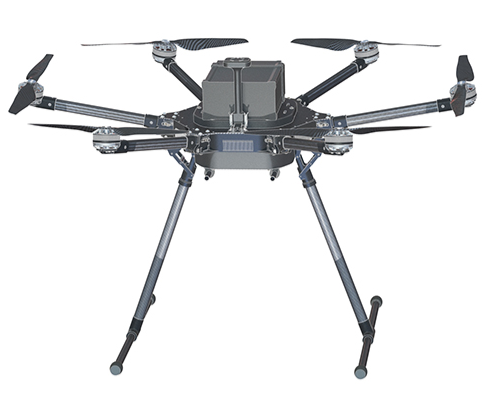
\includegraphics[width=1cm]{images/IF1200.png} & 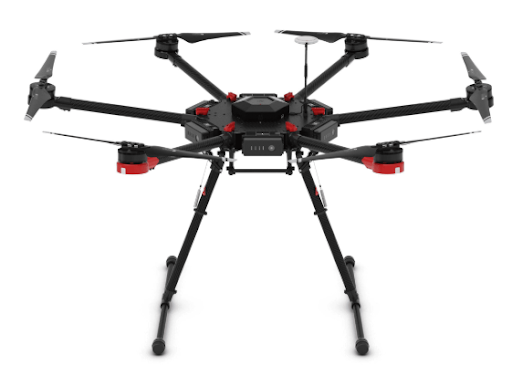
\includegraphics[width=1cm]{images/DJI.png} & 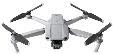
\includegraphics[width=1cm]{images/mavic.jpeg} & 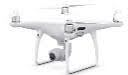
\includegraphics[width=1cm]{images/phantom.jpeg} \\ 
\hline
\textbf{Aircraft} & \textbf{Inspired Flight (USA)} & \textbf{DJI} & \textbf{DJI} & \textbf{DJI} \\ 
\hline
\textbf{Model} & IF 1200 & Matrice 600 & Phantom 4 Pro V2 & Mavic Air 2 \\ 
\hline
\textbf{Type} & VTOL & VTOL & VTOL & VTOL \\ 
\hline
\textbf{Use} & Payload Carrier, Red Target & Red Target & Red Target & Red Target \\ 
\hline
\end{tabular}%
}
\caption{Escape II Data Collection SUAS devices deployed}
\label{table:aircraft}
\end{table}
\end{frame}

\begin{frame}{Non-negative matrix factorization (NMF)}

\begin{block}{Problem Statement}
Given a non-negative matrix $V \in \mathbb{R}^{m \times n}$, find non-negative matrices $W \in \mathbb{R}^{m \times r}$ and $H \in \mathbb{R}^{r \times n}$ such that:
\[ V \approx WH \]
where $r$ is the rank of the factorization
\end{block}

\begin{block}{Interpretation}
\begin{itemize}
\item $W$ represents a basis matrix:
  \begin{itemize}
  \item Each column of $W$ represents a basis vector in the space of the original data $V$
  \end{itemize}
\item $H$ represents a coefficient matrix:
  \begin{itemize}
  \item Each column of $H$ represents the temporal activation coefficients to express the corresponding basis vector
  \end{itemize}
\end{itemize}
\end{block}
\end{frame}

\begin{frame}{NMF For Audio Source Separation}
\begin{itemize}
    \item Used to decompose the original signal into $N$ spectral components, each capturing a relevant feature
    \item The dot product of \( W \) and \( H \) yields an approximation of \( V \):
    \[
    W \odot H \approx V
    \]
    \item NMF allows you to select specific spectral components and add/remove them from a recreated signal:
    \[
    V \approx W[:, 1] \cdot H[1, :] + W[:, 2] \cdot H[2, :] + \ldots
    \]
    where \( W[:, j] \) represents the \( j \)-th basis vector and \( H[j, :] \) represents the coefficients for the \( j \)-th basis vector
\end{itemize}
\end{frame}

\begin{frame}{Visualization}
\begin{figure}[h]
    \centering
    \subfigure[First four columns of H (temporal activation coefficients)]{
        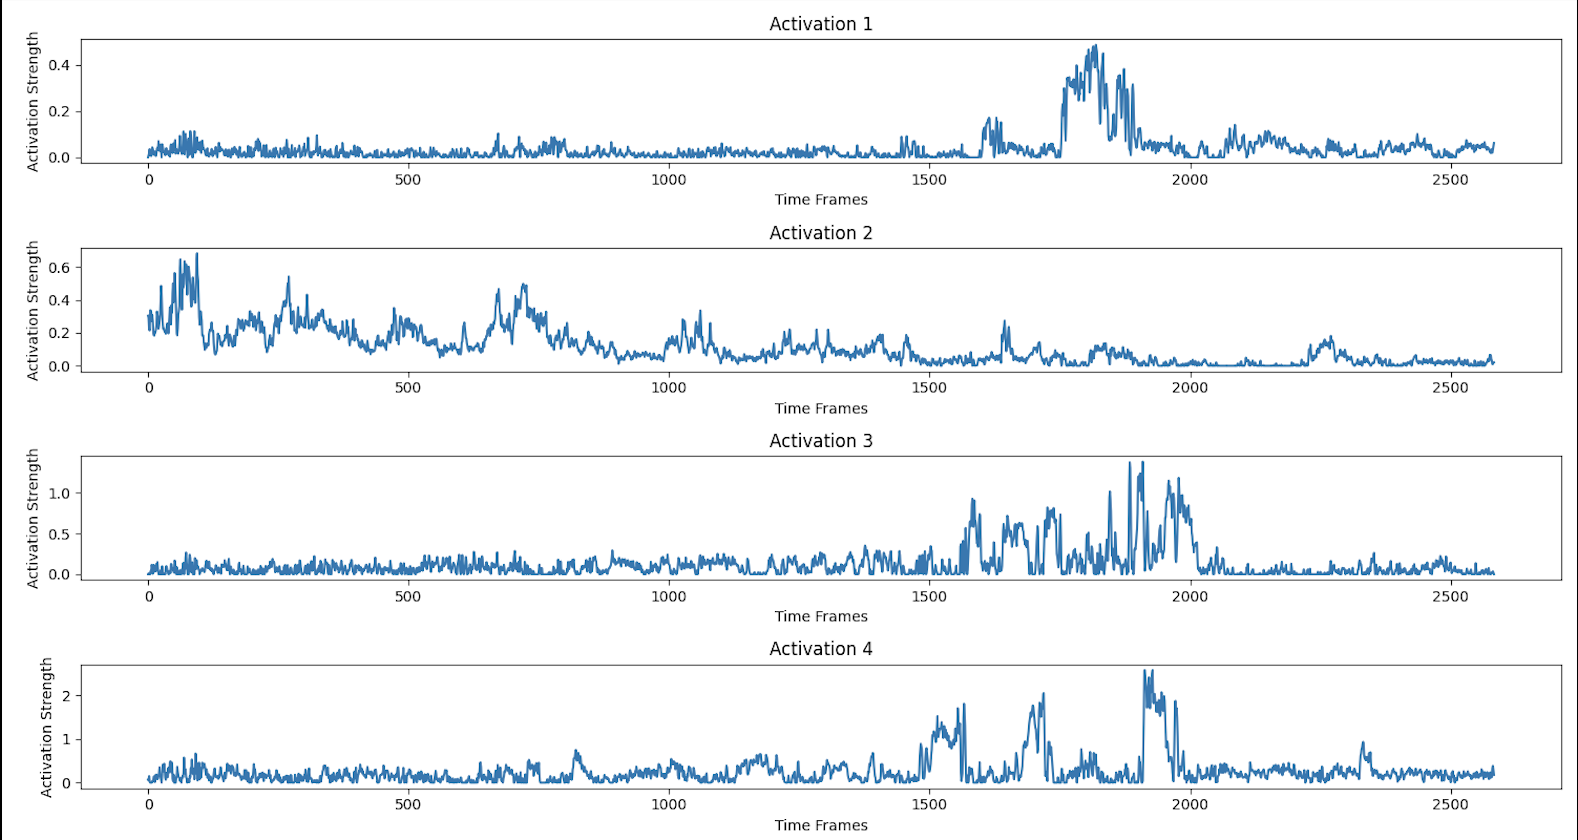
\includegraphics[width=0.5\textwidth]{images/activations.png}
    }
    \hspace{0.05\textwidth}
    \subfigure[First four basis vectors of W]{
        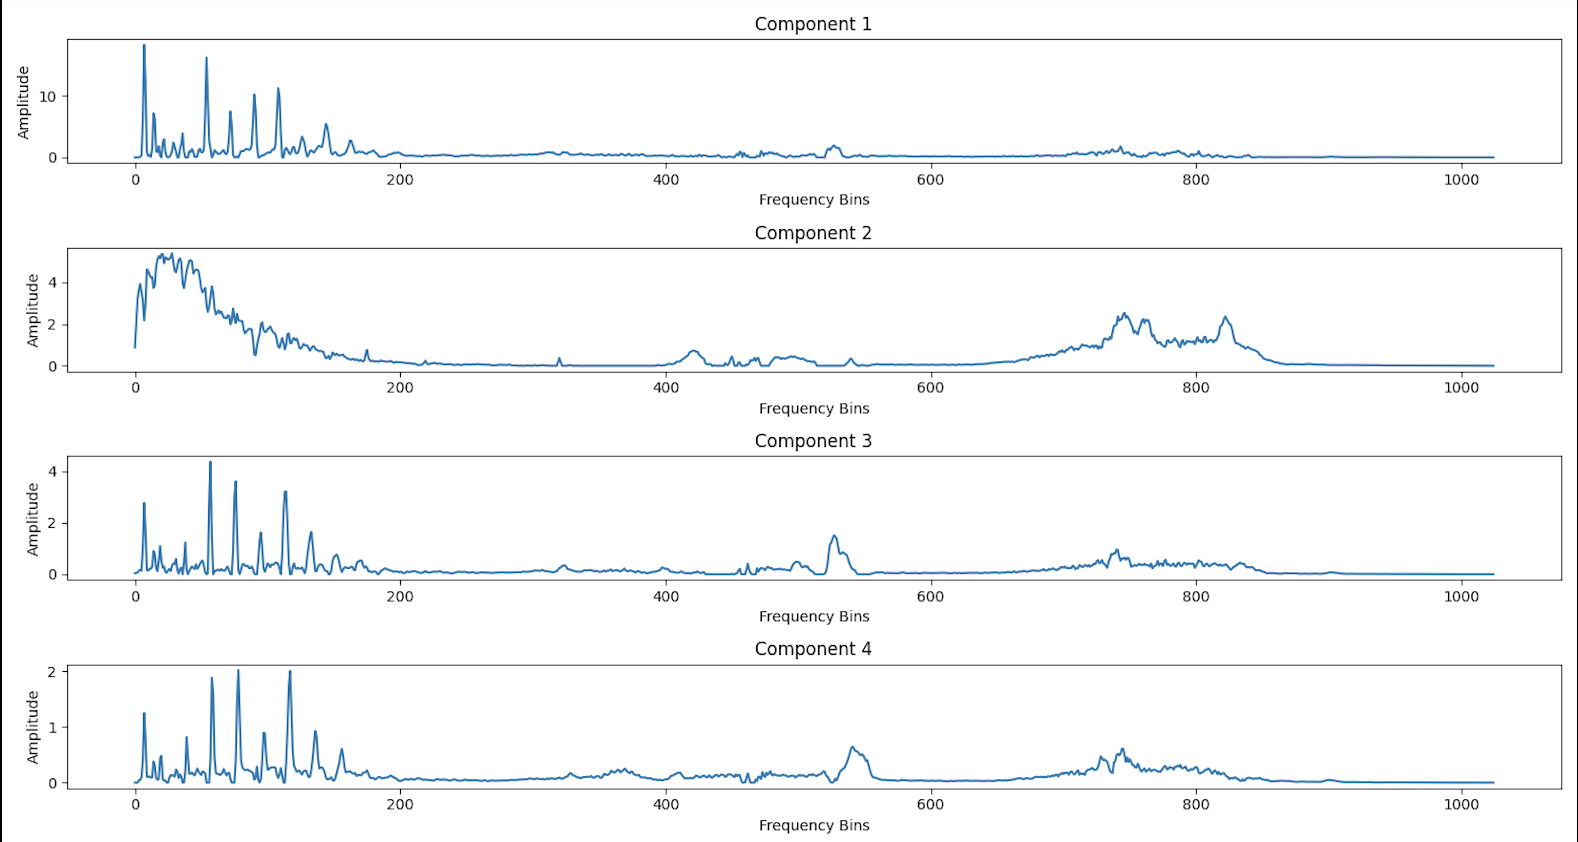
\includegraphics[width=0.5\textwidth]{images/components.png}
    }
    
\end{figure}
\end{frame}

\begin{frame}{Non-negative Matrix Factorization (NMF) Optimization}

The goal of NMF is to minimize the difference between the original matrix $V$ and the product of the basis matrix $W$ and the coefficient matrix $H$. This is typically achieved by minimizing a cost function, such as the Frobenius norm of the difference:

\begin{equation*}
\min_{W,H} \frac{1}{2} ||V - WH||_F^2 \quad \text{subject to} \quad W,H \geq 0
\end{equation*}

The optimization problem is solved using iterative update rules for $W$ and $H$:

\begin{align*}
H_{ij} &\leftarrow H_{ij} \frac{(W^T V)_{ij}}{(W^T W H)_{ij}} \\
W_{ij} &\leftarrow W_{ij} \frac{(V H^T)_{ij}}{(W H H^T)_{ij}}
\end{align*}

These update rules are applied alternately until convergence or a maximum number of iterations is reached. The non-negativity constraints on $W$ and $H$ ensure that the factorization yields interpretable and meaningful components.

\begin{figure}[h]
    \centering
    \textbf{Flowchart goes here}
    \includegraphics[width=0.8\textwidth]{images/nmf_optimization.png}
    \caption{Schematic representation of the NMF optimization process.}
\end{figure}

\end{frame}

\begin{frame}{NMF for Audio Source Separation}

In the context of audio source separation, NMF is applied to the magnitude spectrogram of the audio signal. The spectrogram is obtained by performing a Short-Time Fourier Transform (STFT) on the time-domain signal:

\begin{equation*}
V = |\text{STFT}(x)|
\end{equation*}

where $x$ is the time-domain audio signal and $V$ is the resulting magnitude spectrogram.

NMF decomposes the spectrogram into a set of spectral basis vectors $W$ and their corresponding temporal activation coefficients $H$:

\begin{equation*}
V \approx WH
\end{equation*}

Each basis vector in $W$ captures a specific spectral pattern, while the corresponding row in $H$ represents the temporal activation of that pattern.

To separate specific sources or remove noise, relevant basis vectors can be selected and used to reconstruct a modified spectrogram:

\begin{equation*}
\tilde{V} = \sum_{j \in J} W_{:,j} H_{j,:}
\end{equation*}

where $J$ is the set of indices corresponding to the selected basis vectors. The modified spectrogram $\tilde{V}$ can then be used to synthesize the separated or denoised audio signal using the inverse STFT.

\begin{figure}[h]
    \centering
    \textbf{Flowchart goes here}
    \includegraphics[width=0.8\textwidth]{images/nmf_audio_separation.png}
    \caption{Overview of the NMF-based audio source separation process.}
\end{figure}

\end{frame}

\begin{frame}{Matrix Embedding and Optimization [IN PROGRESS]}
The generalized noise type matrices are first horizontally concatenated to form a noise basis matrix $W_\text{noise}$:
\begin{equation*}
W_\text{noise} = [W_{\text{type}1} ; W_{\text{type}2} ; W_{\text{type}3}]
\end{equation*}
where $W_{\text{type}_i}$ represents the basis matrix for the $i$-th noise type.
The noise basis matrix $W_\text{noise}$ is then embedded into a larger basis matrix $W$ along with randomly initialized signal basis vectors $W_\text{signal}$:
\begin{equation*}
W = \left[\begin{array}{c|c}
\boxed{W_{\text{type}1}} \boxed{W_{\text{type}2}} \boxed{W_{\text{type}3}} & \boxed{W_\text{signal}} \\
\end{array}\right]
\end{equation*}
\begin{minipage}{0.6\textwidth}
The corresponding activation matrix $H$ is also initialized with \textit{entirely} random values:
\end{minipage}
\hfill
\begin{minipage}{0.3\textwidth}
\begin{equation*}
H = \left[\begin{array}{c}
\boxed{H_\text{noise}} \\
\
\boxed{H_\text{signal}}
\end{array}\right]
\end{equation*}
\end{minipage}
During the optimization process, the signal basis vectors $W_\text{signal}$ and the entire activation matrix $H$ are updated iteratively using the multiplicative update rules, while the noise basis vectors $W_\text{noise}$ remain fixed:
\begin{align*}
H &\leftarrow H \odot \frac{W^T V}{W^T (W H)} \ & W_\text{signal}\leftarrow W_\text{signal} \odot \frac{V H_\text{signal}^T}{(W H) H_\text{signal}^T}
\end{align*}
where $\odot$ represents element-wise multiplication and division.
By fixing the noise basis vectors and optimizing only the signal basis vectors and activation matrix, the algorithm aims to separate the noise and drone signals effectively.
\end{frame}

%%%%%%%%%%%%%%%%%%%%%%%%%%%%%%%%%%%%%%%%%%%%%%%%%%%%%%%%%%%%%

\section{Future Work}

\begin{frame}{Future Work}

\begin{itemize}
    \item Perform unsupervised clustering on the data
    \item Refine NMF-based approach to enhance SUAS signature and reduce noise 
    \item Modify NMF loss function to handle the frequency and time dimensions differently, prevent bleeding in the time domain
    \item Change the transform used prior to NMF from STFT -> Orthogonal Mode Decomposition
\end{itemize}

\begin{block}{Overarching Goals}
    \begin{itemize}
        \item Develop a robust and automated noise removal algorithm to enhance SUAS detection and classification via machine learning
        \item Deploy a CNN for classifying the specific SUAS device present in a given audio signal. Eventually, use a rank-3 tensor convolution for spatial data fusion.
        \item Explore techniques to confound machine learning models trained to detect and classify SUAS devices
        \item Investigate GANs and the potential to generate synthetic SUAS or noise signals when paired with the NMF approach
    \end{itemize}
\end{block}
\end{frame}

%%%%%%%%%%%%%%%%%%%%%%%%%%%%%%%%%%%%%%%%%%%%%%%%%%%%%%%%%%%%%

\end{document}
